\subsubsection{DC-Motor}
Der DC-Motor dient dem Vorschub der Bälle. Diese werden so dem
Abwurfmechanismus zugeführt, welche dieser dann selbstständig
greift und mittels des Schwungrades abwirft. Hierzu wird ein
einfacher und kräftiger Bürstenmotor verwendet vom Typ Xdrive
555-1 der Marke Motraxx.

\begin{figure}[h!]
	\centering
	\begin{subfigure}[b]{0.45\textwidth}
		\centering
		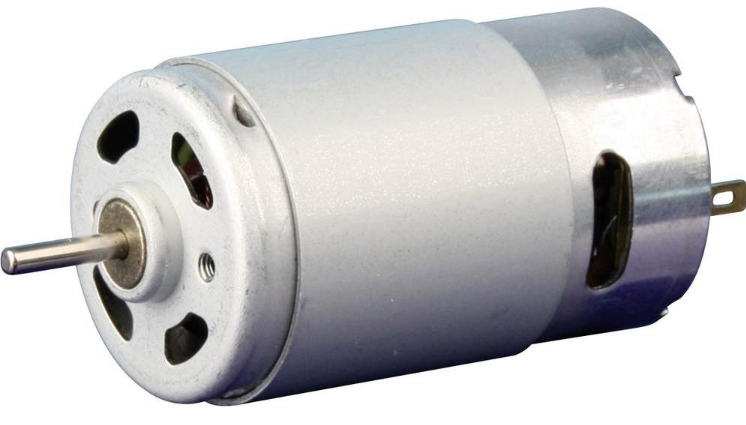
\includegraphics[width=1\textwidth]{../../fig/et/dc_01.png}
		\caption{Gleichstrommotor Xdrive 555-1 von Motraxx}
	\end{subfigure}
	\begin{subfigure}[b]{0.45\textwidth}
		\centering
		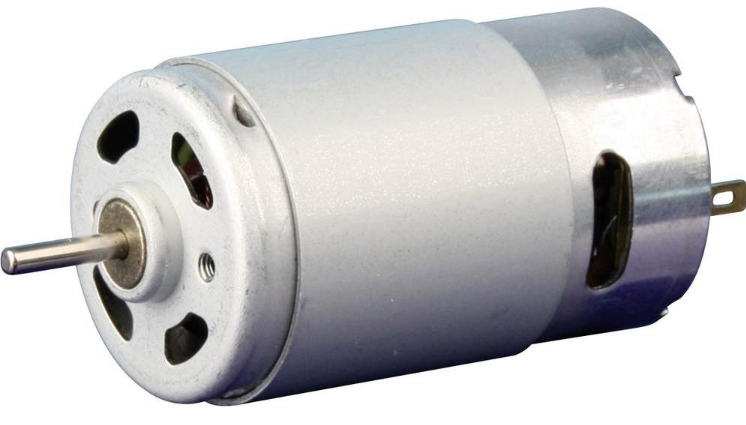
\includegraphics[width=1\textwidth]{../../fig/et/dc_01.png}
		\caption{DC-Treiberboard der Gruppe PREN-ET}
	\end{subfigure}
	\caption{Motor und Elektronik des Ballvorschubs}
\end{figure}

Für die Ansteuerung des DC-Motors wird ein eigens in der Gruppe
PREN-ET entwickeltes Board verwendet. Dieses beinhaltet als
Kernelement den Treiberchip A3941 von Maxim. Dieser bietet die
Möglichkeit das PWM Signal einzuspielen und so die gemittelte
Motorspannung zu stellen. Diese wird mittels einer
MOSFET-Vollbrücke über dem Motor eingestellt. Für die vorliegende
Implementierung ist dabei die externe PWM Vorgabe deaktiviert.
Dieses wird on-board erzeugt und ist mittels eines
Trimmpotentiometers eingestellt. Das so konfigurierte Board
bietet nun ein einfaches Interface welches lediglich zwei
Eingangssignale kennt: Enable (Ein / Aus) und Direction (Aufwärts
/ Abwärts).
%
%\begin{itemize}
%	\item Enable \hfill{Ein / Aus}
%	\item Direction \hfill{Aufwärts / Abwärts}
%\end{itemize}
%
Die vollständige Dokumentation des Treiberboards ist auf dem
Gruppenrepository \url{https://github.com/pren-et/doc}
von PREN-ET zu finden oder im Anhang \ref{sec:dc_doc} einsehbar.
Die Bedienung des Treiberboards ist vollständig in der Firmware des
Freedomboards implementiert und in der Shell verfügbar. Hierzu kann
das Kommando \verb!DC! verwendet werden.

Eine gekoppelte Komponente stellen jeweils die Endschalter dar.
Diese sind fester Bestandteil der Ansteuerungsfirmware des
Treiberboards und implementiert einige Automatismen zum Schutz
des Motors und zum einwandfreien einsatz des Ballvorschubs.
